% !TeX program = xelatex


\documentclass[10pt,pdf,hyperref={unicode}]{beamer}
\usetheme{Frankfurt}

\usepackage{xltxtra} 
\usepackage{fontspec}
\usepackage{polyglossia} % поддержка языков (вместо babel)  

\usepackage[normalem]{ulem} % выдление подчеркиванием и зачеркиванием (\uline{}, \uwave{})
% но стандартную команду \emph{text} не переопределяем

\usepackage{graphicx}
\graphicspath{ {./pic/} }
\setdefaultlanguage[spelling=modern]{russian} 
\setkeys{russian}{babelshorthands=true}
% babel shorthands are:
%  "--- Cyrillic emdash in plain text.
%  "--~ Cyrillic emdash in compound names (surnames).
%  "--* Cyrillic emdash for denoting direct speech.
% "~ неразрывный дефис. Пример: как в 90"~х годах

\setotherlanguage{english}
\defaultfontfeatures{Renderer=Basic, Ligatures=TeX} %лигатуры работают в basic режиме
% \defaultfontfeatures{Scale=MatchLowercase, Mapping=tex-text} 

\setmainfont{Times New Roman}
\setsansfont{Arial}
\setmonofont{Courier New}
\newfontfamily{\cyrillicfonttt}{Courier New} 

\usepackage{tikz}
\usetikzlibrary{graphs,shapes,arrows}



\newcommand{\Enl}[1]{\textbf{\large#1}}

\title{Знакомство с LaTeX}
\author{Илья Кочергин}
\institute{кафедра экономической информатики} 
\titlegraphic{
\includegraphics[width=4cm]{EF_logo_and_title}%
}
\begin{document}
    
\section*{титульный слайд}    
    
    
\begin{frame}
\titlepage
\end{frame}

\section{Что такое LaTeX}
\begin{frame}
     \frametitle{Что такое \LaTeX?}
     \begin{itemize}
         \item Произносится Лэйтек или Латех (как \textbf{тех}нология)
         \item Система вёрстки научных статей и презентаций
         \item Язык разметки (Markup) наряду с 
         \begin{itemize}
             \item HTML
             \item Markdown
             \item XML
            \end{itemize}
         \item Стандарт де-факто для набора математических и химических формул
         \item Основан на системе компьютерной типографии \TeX{} 
      \end{itemize}
\end{frame}

\begin{frame}[shrink]
    \frametitle{Что применять язык  или графический интерфейс?}
    \begin{block}{WYSIWYG - What You See Is What You Get}
      \begin{itemize}
          \item Microsoft Word, Powerpoint, Excel
          \item Позволяют не запоминать море технической информации 
          \item Хороши при эпизодическом использовании 
          \item Кривая отдачи от обучения (Learnig Curve) имеет пологий участок в конце 
          \item При написании текста мы всё время отвлекаемся на оформление
        \end{itemize}
        
    \end{block}
    
    \begin{block}{Языки разметки и программирования}
        \begin{itemize}
            \item \LaTeX{}, R, Python
            \item Занимают много места в голове человека  
            \item Хороши при каждодневном использовании 
            \item Кривая отдачи от обучения (Learnig Curve) имеет пологий участок в начале
            \item \LaTeX{} позволяет во время написания документа или презентации сосредоточится на содержании, доверив системе оформление 
        \end{itemize}     
    \end{block}
    
\end{frame}
\section{Кто сделал наибольший вклад в создание \LaTeX{}? }
\begin{frame}
\frametitle{Дональд Кнут в 1978 году придумал \TeX}
    \begin{columns}[c]
    \begin{column}{0.5\textwidth}
       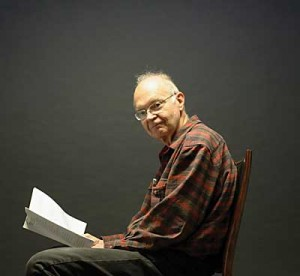
\includegraphics[keepaspectratio,height=0.5\textheight]{knuth.jpg}
    \end{column}
    \begin{column}{0.5\textwidth}
    \begin{itemize}
        \item Математик из Стэндфордского университета
        \item Автор 10-томного  <<The Art of Computer Programming>>
        \item Почётный член многих академий, в том числе, РАН
    \end{itemize}
    \end{column}
  \end{columns}
  \vfill
    \begin{itemize}
        \item[\TeX{}] --- компилятор низкоуровневого языка форматирования текста  и основа для \LaTeX{},  Plain\TeX{}, Con\TeX{}t и других высокоуровневых  надстроек.
        \item[\TeX{}] вобрал огромный массив знаний, накопленных в книгоиздательском деле.
    \end{itemize}
\end{frame}
\begin{frame}
    \frametitle{Лесли Лэмпорт в 1984 году придумал \LaTeX}
    \begin{columns}[c]
        \begin{column}[c]{0.5\textwidth}
            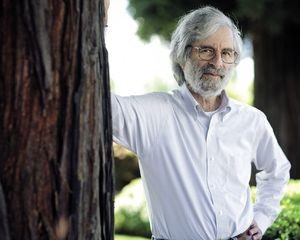
\includegraphics[keepaspectratio,width=0.95\textwidth]{lamport.jpg}
        \end{column}
        \begin{column}[c]{0.5\textwidth}
            \begin{itemize}
                \item Работал в MIT, сейчас работает в Microsoft
                \item Лауреат премии имени Тьюринга (в области информатики это аналог Нобелевской премии) 
            \end{itemize}
        \end{column}
    \end{columns}
    \vfill
   \begin{itemize}
       \item[\LaTeX{}] --- компилятор высокоуровневого  языка разметки, написанный на  языке \TeX{}.
       \item[\LaTeX{}] --- стандарт де"~факто для вёрстки научных текстов и презентаций.
    \end{itemize}    
\end{frame}

\begin{frame}
    \frametitle{Тиль Тантау придумал Beamer и TikZ}
    \begin{columns}[c]
        \begin{column}{0.5\textwidth}
            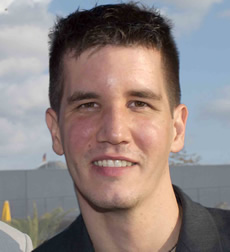
\includegraphics[keepaspectratio,height=0.5\textheight]{till_tantau.jpg}
        \end{column}
        \begin{column}{0.5\textwidth}
            \begin{itemize}
                \item Работает в университете города Любек, Германия
                \item Специалист в области информатики  
            \end{itemize}
        \end{column}
    \end{columns}
    \vfill
    \begin{itemize}
        \item[TikZ] --- подъязык для создания диаграмм и графиков функций, реализованный в \TeX{} как пакет. TikZ расшифровывается рекурсивно: "TikZ ist kein Zeichenprogramm"  (TikZ --- это не программа для рисования).
        \item[Beamer] --- класс документов \LaTeX{} для создания презентаций. Beamer "--- псевдо-английское слово, обозначающее по-немецки проектор. 
    \end{itemize}    
\end{frame}


\begin{frame}
	\frametitle{Что за БИВНИ?}

\begin{columns}
	\begin{column}{0.4\textwidth}
		\begin{itemize}
            \vfill 
			\item[\Enl{Б}]азовые 
			\item[\Enl{И}]нструменты 
			\item[\Enl{В}]оспроизводимых 
			\item[\Enl{Н}]аучных 
			\item[\Enl{И}]сследований
		\end{itemize}
	\end{column}
	\begin{column}{0.6\textwidth}
		\onslide*<1> {
	%	\vspace{1cm}	
		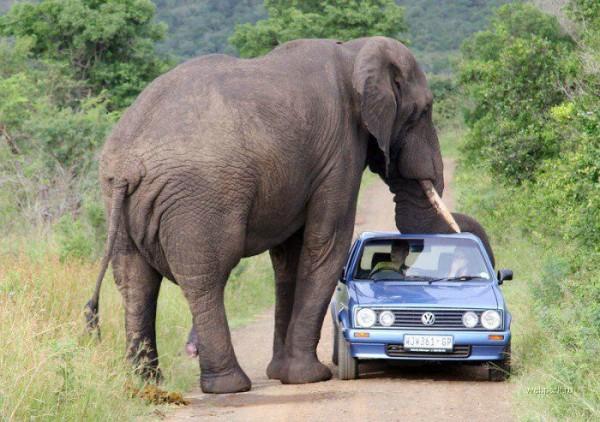
\includegraphics[scale=0.3]{ataka-slona-600x422.jpg}}
		\onslide*<2->{
		\begin{itemize}
			\item[\Enl{R}]eproducible 
			\item[\Enl{R}]esearch
		\end{itemize} }
	\end{column}
    \begin{column}{0.6\textwidth}
      \onslide*<2->{
        \begin{itemize}
            \item \textbf{\LaTeX}
            \item \textbf{R} 
        \end{itemize} %
      }  
        
       \end{column}	
\end{columns}	
\end{frame}


 
    

%\begin{frame}
%\frametitle{\secname}
%    
%    \begin{columns}[T]
%        \centering
%        
%        \begin{column}{0.5\textwidth}
%                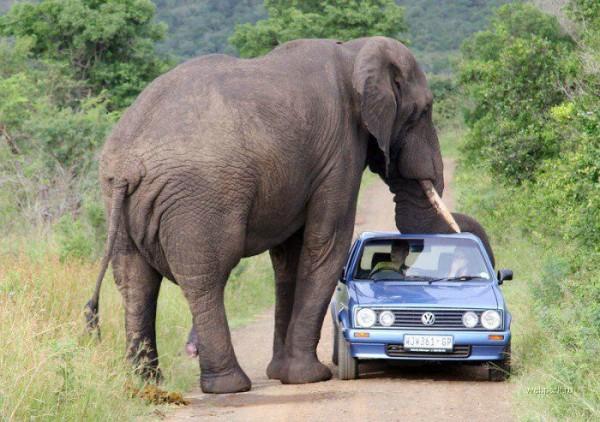
\includegraphics[width=0.99\textwidth,height=0.8\textheight,keepaspectratio]{ataka-slona-600x422.jpg}
%                
%                Это слон 
%        \end{column}
%        \begin{column}{0.5\textwidth}
%                 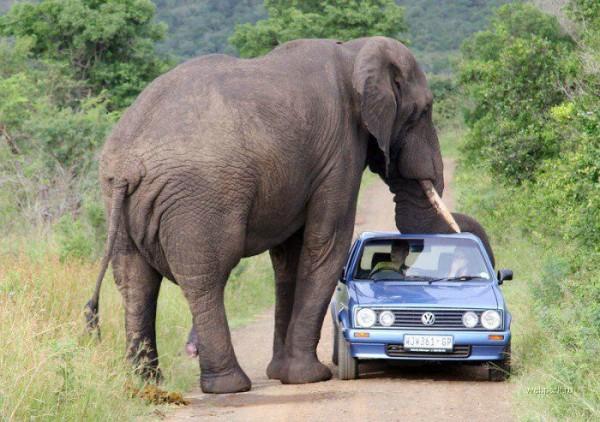
\includegraphics[width=0.99\textwidth,keepaspectratio]{ataka-slona-600x422.jpg}
%                 
%                  \twophoto{arg1}{arg2}{arg3}{arg4}        
%         \end{column}	
%        \end{columns}	
%\end{frame}





\begin{frame} 
	\frametitle [Зачем нужна воспроизводимость] {Зачем нужна воспроизводимость научных исследований }
\begin{itemize}
\item Возможность выявить ошибки, воспроизводя этапы работы с данными  
\begin{itemize}
	\item[-] Результаты исследований ложатся в основу экономических решений и законов (порядок цены~$\$10^{10})$
	\item[-] Данные и многоэтапные  вычисления, на которые опирается исследования могут содержать ошибки
\end{itemize}
\item  Распространение знаний
    \begin{itemize}
       \item[-] возможность изучить методику автора научной публикации
       \item[-] можно увидеть формулы и алгоритмы работы с данными  
    \end{itemize}
    
\end{itemize}
\end{frame}	

\end{document}
